\documentclass[upright, contnum]{umemoria}

%fix for the oneside argument
\makeatletter
\g@addto@macro\titlepage{\pagenumbering{Alph}}
\g@addto@macro\endtitlepage{\pagenumbering{roman}}
\makeatother

\depto{Departamento de Ciencias de la Computación}
\author{Matías Ignacio Meneses Cortés}
\title{Type-Based Declassification en Dart: Implementación y Elaboración de Herramientas de Inferencia}
\auspicio{}
\date{Abril 2018}
\guia{Éric Tanter}
\carrera{Ingeniero Civil en Computación}
\memoria{Memoria para optar al Título de \break  Ingeniero Civil en Computación}
\comision{}

\usepackage{lipsum}

\usepackage[utf8]{inputenc}
\usepackage[T1]{fontenc}
\usepackage{color}

\definecolor{dkgreen}{rgb}{0,0.6,0}
\definecolor{gray}{rgb}{0.5,0.5,0.5}
\definecolor{mauve}{rgb}{0.58,0,0.82}

\usepackage{listings}
\lstset{%
	basicstyle=\large,
	numberstyle=\tiny,
	numbersep=15pt,tabsize=4,
	flexiblecolumns=true,
	keywordstyle=\color{blue},
	commentstyle=\color{dkgreen},
	stringstyle=\color{mauve},
	numberstyle=\tiny\color{gray},
	language=Java,
	breaklines=true,
	breakatwhitespace=true,
  showstringspaces=false,
  aboveskip=1.2em,
  belowskip=1.2em,
	morekeywords={*,num,String,var,library,get,set} ,
}

\begin{document}
\frontmatter
\maketitle

\begin{abstract}
{\lipsum[1-4]}
\end{abstract}

\begin{dedicatoria} % opcional
Una dedicatoria corta. Por ejemplo, \emph{A los creadores de U-Campus}
\end{dedicatoria}

\begin{thanks} % opcional
\lipsum[1-2]
\end{thanks}
\cleardoublepage

\tableofcontents
\listoftables % opcional
\listoffigures % opcional

\mainmatter

\begin{intro}

	La protección de la confidencialidad de la información manipulada por los programas computacionales es un problema cuya relevancia se ha incrementado en el último tiempo, a pesar de tener varias décadas de investigación. Por ejemplo, una aplicación web (o móvil) que como parte de su funcionamiento debe interactuar con servicios de terceros y por tanto debe proteger que su información sensible no se escape durante la ejecución de la aplicación a canales públicos.

	Muchas de las técnicas de seguridad convencionales como \textit{control de acceso} tienen deficiencias para proteger la confidencialidad de un programa, por ejemplo no restringen la propagación de información\cite{myers-phd}.

	Formas más expresivas y efectivas de proteger la confidencialidad se basan en un análisis estático sobre el código del programa, y se categorizan dentro de \textit{language-based security}. Una de las técnicas más efectivas se denomina \textit{tipado de seguridad} en un \textit{lenguaje de seguridad}, donde los tipos son anotados con niveles de seguridad para clasificar la información manipulada por el programa.

	Uno de los mayores desafíos de los lenguajes de seguridad es facilitar el trabajo del programador, utilizando técnicas más expresivas. En esta dirección, Cruz et al.~\cite{cruzAl:ecoop2017} recientemente propusieron \textit{type-based declassification}, una variación de tipado de seguridad que utiliza el sistema de tipos del lenguaje para controlar la declasificación de la información.

	\textit{Type-based declassification} presenta limitaciones en cuanto a su implementación, debido a que el análisis teórico se realiza sobre un lenguaje minimalista que no incluye características básicas de los lenguajes de programación, como instrucciones condicionales y mutabilidad. En este trabajo, se propone una extensión al lenguaje minimalista utilizado en \textit{type-based declassification}, y la implementación en el lenguaje de programación Dart, desarrollando un plugin para los editores de texto más populares, con el objetivo de proporcionar una experiencia interactiva e intuitiva al usuario.



		\section{Motivación}
	El tema escogido se considera interesante debido a su importancia teórica y práctica en el campo de la seguridad en lenguajes de programación. Los fundamentos teorícos de \textit{type-based declassification} están bien descritos~\cite{cruzAl:ecoop2017}, pero no así su realización práctica, siendo esto reconocido por sus autores.

	Se considera que la realización de este trabajo es relevante para demostrar y materializar en un lenguaje de uso general la investigación de type-based declassification. Dicha materalización constituye un desafío importante en términos de complejidad, al tener que entender la teoría subyacente de tipado de seguridad, así como extender un lenguaje real y sus herramientas de análisis estático con nuevas funcionalidades.

		\section{Objetivos}
	El objetivo de la memoria es realizar la implementación de un sistema de inferencia para \textit{type-based declassification}. Dentro de los objetivos específicos del trabajo, podemos encontrar:

	\begin{itemize}
	\item \textbf{Inferencia y verificación estática de type-based declassification}. Se entiende coma la implementación de un sistema de inferencia de facetas de declasificación para \textit{type-based declassification}, en el lenguaje de programación Dart. Dentro del análisis de la inferencia se incluye la verificación de las reglas del sistema de tipos de \textit{type-based declassification}.

	\item \textbf{Plugin para editores}. Mostrar al programador el resultado de la inferencia, por medio de un plugin para los editores de texto que soporten servidores de análisis estático de Dart, ofreciéndole acciones al respecto.

	\end{itemize}

		\section{Resultados y Organización del documento}

	En términos concretos este trabajo presenta el diseño de un plugin que realiza el análisis de type-based declassification. Los antecedentes teóricos necesarios para entender este trabajo se abordan en el capítulo 2, mientras que la propuesta de solución es desarrollada en el capítulo 3.

	Los detalles de diseño de implementación de la propuesta son revisados en el capítulo 4.

	% TODO
	Por terminar.


\end{intro}

\chapter{Antecedentes}
En este capítulo se presentan los antecedentes y conceptos teóricos necesarios para entender este trabajo, y se divide en dos secciones principales. La primera, presenta los conceptos de control de flujo de información, mientras que la segunda, presenta los conceptos de inferencia de tipos.
\section{Control de flujo de información} \label{controlflujo}
Los lenguajes con tipado de seguridad para el control del flujo de la información clasifican los valores de un programa con respecto a sus niveles de confidencialidad, expresado mediante una \emph{lattice}\footnote{Un orden parcial, donde todo par de elementos tiene un único supremo e ínfimo} de etiquetas de seguridad. Por ejemplo, con la lattice de dos niveles de seguridad \texttt{L} $\sqsubseteq$ \texttt{H} se puede distinguir entre valores públicos o de baja confidencialidad (\texttt{L}) y valores privados o de alta confidencialidad (\texttt{H}). Un sistema de tipos con control de flujo asegura de forma estática el cumplimiento de la propiedad \emph{noninterference}~\cite{noninterference}, esto es, que la información confidencial no fluya directa o indirectamente hacia canales públicos~\cite{volpanoAl:S96}.

En el siguiente ejemplo se muestra un código anotado con niveles de seguridad, en donde el parámetro \texttt{guess} y el retorno del método se declaran de baja confidencialidad, y el parámetro \texttt{password} se declara de alta confidencialidad.

\begin{ej} \ \\
  \normalfont
  \label{ej2-1}
\begin{lstlisting}
  bool@L login(String@L guess, String@H password) {
    return password == guess;
  }
\end{lstlisting}
\end{ej}

En el ejemplo \ref{ej2-1} ocurrió un \emph{flujo explícito}, debido a que un observador público puede obtener información del parámetro confidencial \texttt{password} observando las salidas del programa, lo que no ocurriría si \texttt{login} declara un retorno de tipo \texttt{bool@H}.

Un flujo explícito significa una infracción a noninterference. Para su detección, los lenguajes de seguridad poseen distintas reglas que relacionan los niveles de seguridad involucrados. En una instrucción de asignación \texttt{x = y}, se dice que el nivel de seguridad de \texttt{y} debe ser igual o menor que el nivel de seguridad de \texttt{x}. En una instrucción de retorno \texttt{return y}, se dice que el nivel de seguridad de \texttt{y} debe ser igual o menor que el nivel de seguridad declarado como retorno del método. En el ejemplo \ref{ej2-1}, el nivel de seguridad de la comparación es \texttt{H}, debido a la propagación del nivel de seguridad de \texttt{password} en la operación de comparación. Esto es mayor que el nivel de seguridad de retorno \texttt{L}.

En el siguiente ejemplo se introduce una variable global al ejemplo \ref{ej2-1} para almacenar el valor de retorno, y se cambia el tipo de retorno de la función por \texttt{void}. Además, se considera que los valores literales son de baja confidencialidad.

\begin{ej} \ \\
  \normalfont
  \label{ej2-12}
\begin{lstlisting}
  String@L ret = "";
  void login(String@L guess, String@H password) {
    if (password == guess) ret = "Login successful";
    else ret = "Login failed";
  }
\end{lstlisting}
\end{ej}

En el ejemplo \ref{ej2-12} ocurrió un \emph{flujo implícito}, debido a que un observador público puede obtener información del parámetro confidencial \texttt{password} observando cambios en el valor que contiene la variable \texttt{ret}, mediante el control de flujo del programa.

Un flujo implícito también significa una infracción a noninterference. Es posible detectar un flujo implícito considerando que las instrucciones de retorno y asignación de valores de baja confidencialidad, ocurren en un contexto de alta confidencialidad, determinado por la condición de la instrucción \texttt{if}. Para considerar el contexto de ejecución de una instrucción en las reglas del sistema de tipos, se utiliza el concepto de \textit{program counter} (\texttt{pc}) para seguridad~\cite{pc}. Así, en el ejemplo \ref{ej2-12} las instrucciones de asignación son inválidas, debido a que asignan valores de baja confidencialidad cuando el \texttt{pc} tiene un valor de alta confidencialidad.

A pesar de que noninterference es una propiedad atractiva para la especificación de sistemas seguros, se considera muy estricta en la práctica, debido a que impide que la información confidencial tenga cualquier tipo de influencia en una salida observable de un programa. En efecto, queremos que el programa de \texttt{login} sea aceptado a pesar de infringir noninterference, pues de otra forma no tendríamos cómo realizar la autenticación.

Para solucionar este problema, los lenguajes de seguridad adicionan mecanismos de \emph{desclasificación} que disminuyen el nivel de seguridad de un valor confidencial, implementados de diferentes formas~\cite{sabelfeldSands:JCS09}. Una de ellas, por ejemplo en Jif~\cite{jif} es usar un operador \texttt{declassify}, que desclasifica un valor de alta confidencialidad retornando un valor de baja confidencialidad. En el ejemplo \ref{ej2-2}, se utiliza para desclasificar el resultado de la operación de comparación.
\clearpage
\begin{ej} \ \\
  \normalfont
  \label{ej2-2}
\begin{lstlisting}
  String@L login(String@L guess, String@H password) {
    if (declassify(password == guess)) return "Login Successful";
    else return "Login failed";
  }
\end{lstlisting}
\end{ej}


A pesar de que este programa no cumple con noninterference, no representa una amenaza de seguridad, debido a que el resultado de la operación de comparación es negligible con respecto al parámetro privado \texttt{password}. Sin embargo, usos arbitrarios del operador \texttt{declassify} pueden resultar en serias fugas de información. Por ejemplo, \texttt{declassify(password)} puede dar conocimiento absoluto sobre el valor de la variable a un observador público.

Varios mecanismos se han explorado para controlar el uso de desclasificación, y poder asegurar además una propiedad de seguridad para el programa~\cite{sabelfeldSands:JCS09}. En esta dirección, Cruz et al.~\cite{cruzAl:ecoop2017} recientemente propusieron \emph{type-based declassification} como un mecanismo de desclasificación que conecta la abstracción de tipos con una forma controlada de desclasificación, en una manera intuitiva y expresiva, proveyendo garantías formales sobre la seguridad del programa.

En type-based declassification los tipos tienen dos facetas; la faceta privada, que refleja el tipo de implementación, y la faceta pública, que refleja las operaciones de desclasificación sobre los valores de dicho tipo. Por ejemplo, el tipo $\mathtt{StringEq} \triangleq [\mathtt{eq} : \mathtt{String} \rightarrow \mathtt{Bool}]$\footnote{La notación $t_1\rightarrow t_2$ corresponde al tipo de una función con parámetro de tipo $t_1$ y retorno de tipo $t_2$} autoriza la operación \texttt{eq} sobre un \texttt{String}. Entonces se puede usar el tipo de dos facetas \texttt{String<StringEq} para controlar la operación de desclasificación de la igualdad sobre \texttt{password}, lo que se muestra en el ejemplo \ref{ej2-3}
\begin{ej} \ \\
  \normalfont
  \label{ej2-3}
\begin{lstlisting}
  String<String login(String<String guess, String<StringEq password) {
  	if (password.eq(guess)) return "Login successful";
  	else return "Login failed";
  }
\end{lstlisting}
\end{ej}


En type-based declassification, se cumple que la faceta privada es subtipo de la faceta pública. En el ejemplo \ref{ej2-3}, \texttt{String} es subtipo de \texttt{StringEq}, relación que se escribe como \texttt{String <: StringEq}. Los tipos que cumplen con esta relación se denominan \emph{well-formed}.

Al igual que en tipado de seguridad de dos o más niveles, las facetas de type-based declassification forman una lattice con relaciones de subtyping, lo que se ejemplifica en la figura \ref{l1}, donde \texttt{StringEq} $\triangleq [\mathtt{eq} : \mathtt{String} \rightarrow \mathtt{Bool}]$ y \texttt{StringEqLength} $\triangleq [\mathtt{eq} : \mathtt{String} \rightarrow \mathtt{Bool}, \mathtt{length} : \mathtt{Unit} \rightarrow \mathtt{Int}]$.
\clearpage
	\begin{figure}[ht]
		\centering
		\begin{tikzpicture}[node distance=2.3cm]
			\node(Top) 												{\texttt{Top}};
			\node(StringEq)		[below right of=Top]			{\texttt{StringEq}};
			\node(StringEqLength)      [below of=StringEq]       {\texttt{StringEqLength}};
			\node(String)				[below of=StringEqLength]       {\texttt{String}};
			\node(int)					[below left of=Top] 			{\texttt{int}};
			\draw(Top)      -- (StringEq);
			\draw(Top)      -- (int);
			\draw(StringEq)      -- (StringEqLength);
			\draw(StringEqLength)      -- (String);
		\end{tikzpicture}
		\caption{lattice de subtyping}
    \label{l1}
	\end{figure}

Si la faceta pública coincide con la faceta privada, toda operación sobre el valor estará autorizada. Cuando esto sucede, se refiere usualmente a la faceta pública con \texttt{Bot}, por encontrarse siempre en la parte inferior de la lattice. Cuando se quiere referir a una faceta pública vacía o que no autoriza ninguna operación, se usa \texttt{Top}, por encontrarse en la parte superior de la lattice.

Los métodos declarados en la faceta pública también poseen tipos de dos facetas en sus firmas. Así, el tipo \texttt{StringEq} visto anteriormente se define como $\mathtt{StringEq} \triangleq [\mathtt{eq} : \mathtt{String<String} \rightarrow \mathtt{Bool<Bool}]$.

Existen dos reglas principales para comprobar que un programa con tipos de dos facetas se encuentra bien tipado. Consideremos el siguiente ejemplo, en donde $\mathtt{StringHashEq} \triangleq [\mathtt{hash} : \mathtt{Unit<Unit} \rightarrow \mathtt{String<StringEq}]$.

\begin{ej} \ \\
  \normalfont
  \label{ej2-6}
\begin{lstlisting}
  String<StringEq getHash(String<StringHashEq password) {
  	return password.hash();
  }
\end{lstlisting}
\end{ej}

En el ejemplo \ref{ej2-6}, el valor de retorno de la invocación al método \texttt{hash} sobre el parámetro \texttt{password}, tiene faceta pública \texttt{StringEq}, debido a que fue declarado de esta forma en la faceta pública \texttt{StringHashEq}. A esta regla se le llama \texttt{TmD}.

Ahora consideremos el siguiente ejemplo, en donde se cambia la faceta pública del parámetro \texttt{password} del ejemplo \ref{ej2-6} por \texttt{StringEq}.
\clearpage
\begin{ej} \ \\
  \normalfont
  \label{ej2-7}
\begin{lstlisting}
  String<Top getHash(String<StringEq password) {
  	return password.hash();
  }
\end{lstlisting}
\end{ej}

En el ejemplo \ref{ej2-7} se realiza una invocación al método \texttt{hash} sobre el parámetro \texttt{password}, que declara una faceta pública que no autoriza la operación. Cuando esto sucede, la faceta pública de retorno de la invocación es \texttt{Top}. A esta regla se le llama \texttt{TmH}.

La propiedad de seguridad que se demuestra para el sistema de tipos de type-based declassification es una forma de noninterference con políticas de desclasificación, denominada \emph{Relaxed noninterference}. Un lenguaje de seguridad que cumple esta propiedad, garantiza que la información confidencial sólo puede fluir hacia canales públicos de forma controlada, por medio de las políticas de desclasificación.

\section{Inferencia de tipos} \label{inference}
En la sección anterior se revisaron los conceptos relacionados a control de flujo de información, que sirven para comprender el trabajo de type-based declassification. En esta sección se revisan los conceptos relacionados a inferencia de tipos, necesarios para comprender la propuesta de esta memoria.

La inferencia de tipos es el proceso de determinar el tipo de las expresiones en un programa, basado en cómo son usadas. Tener un mecanismo de inferencia en un lenguaje de programación puede ser muy útil, debido a que da la posibilidad al programador de omitir las declaraciones de tipo para algunos identificadores, y mantener los beneficios de un lenguaje estáticamente tipado.

Para ilustrar los conceptos importantes de inferencia, consideremos un lenguaje sencillo con funciones y operaciones aritméticas sobre enteros, cuya sintaxis se muestra en el siguiente ejemplo.
\vspace{0.8em}
\begin{ej}
  \normalfont
  \label{ej2-8}
\begin{lstlisting}
  let g = (x) => x + 5;
\end{lstlisting}
\end{ej}

En el ejemplo \ref{ej2-8}, \texttt{g} es una función que dado un \texttt{x}, retorna la suma entre \texttt{x} y \texttt{5}. Los lenguajes con inferencia de tipos pueden deducir el tipo de \texttt{g}, que en este caso es $\mathtt{int \rightarrow int}$.

Para razonar sobre tipos desconocidos, los sistemas de inferencia asignan \emph{variables de tipo} a cada expresión con tipo desconocido, y \emph{tipos concretos} a cada expresión con tipo conocido.

\begin{center}
  \ttfamily
  \begin{tabular}{l c}
    Expresión & Tipo \\
    \hline
    (x) =>\ x + 5 & X \\
    x & Y \\
    x + 5 & Z \\
    + & $\mathtt{int \rightarrow int}$ \\
    x & W \\
    5 & int \\
  \end{tabular}
\end{center}


Cuando se procesan las expresiones del programa y se asignan los tipos, se generan condiciones que los tipos deben cumplir para que cada expresión esté bien tipada. Estas condiciones se denominan \emph{constraints}, y en este caso expresan una relación de igualdad entre dos tipos.

El uso de constraints permite presentar un algoritmo de inferencia de forma modular, como una fase de generación de constraints, y una fase de resolución de constraints.

Las siguientes observaciones permiten derivar el \emph{set de constraints} del programa.

\begin{enumerate}
  \item Tenemos una función anónima \texttt{(x) =>\ x + 5} que debe tener tipo $\mathtt{Y \rightarrow Z}$, donde \texttt{Y} es el tipo del parámetro y \texttt{Z} es el tipo del cuerpo.
  \item Tenemos una aplicación de la función suma, por lo que se generan condiciones sobre los argumentos. En este caso, \texttt{W = int}.
  \item El parámetro de la función anónima se utiliza como argumento de la suma, por lo que se genera la constraint \texttt{W = Y}.
  \item Como la suma tiene tipo $\mathtt{int \rightarrow int}$, la aplicación \texttt{x + 5} tiene tipo \texttt{int}. Luego se genera la constraint \texttt{Z = int}.
\end{enumerate}

Sintetizando, el set de constraints generado es el siguiente:

\begin{enumerate}
  \item $\mathtt{X = Y \rightarrow Z}$
  \item \texttt{W = int}
  \item \texttt{W = Y}
  \item \texttt{Z = int}
\end{enumerate}

Una vez que se genera el set de constraints sobre el programa, se procede a encontrar una solución para las variables de tipo del set de constraints. Cuando las constraints son de igualdad, se utiliza el algoritmo de unificación de Damas-Milner~\cite{damasmilner}. Este algoritmo genera un mapeo entre variables de tipo y tipos concretos, mediante substituciones. La solución esperada del ejemplo \ref{ej2-8} es:

\begin{center}
  \ttfamily
  \begin{tabular}{c c}
    Variable de tipo & Tipo concreto \\
    \hline
    X & $\mathtt{int \rightarrow int}$  \\
    Y & int \\
    Z & int \\
    W & int \\
  \end{tabular}
\end{center}
\clearpage
Desafortunadamente, el algoritmo de unificación de Damas-Milner no funciona cuando las constraints son de subtyping. Consideremos una extensión del lenguaje anterior,   en donde se introducen los tipos \texttt{num} y \texttt{float}, donde se cumple \texttt{float <: num} y \texttt{int <: num}. En el ejemplo \ref{ej2-9} se muestran dos instrucciones de asignación.
\vspace{0.8em}
\begin{ej}
  \normalfont
  \label{ej2-9}
\begin{lstlisting}
  let f = 4;
                (...)
                f = 1.5;
\end{lstlisting}
\end{ej}

Las constraints que se generan para las asignaciones a la variable f son:

\begin{enumerate}
  \item \texttt{int <: X}
  \item \texttt{float <: X}
\end{enumerate}

Para resolver relaciones de este tipo, Cardelli~\cite{cardelli} considera la relación de orden parcial entre los tipos, inducida por la relación de subtyping, que se muestra en la figura \ref{subt1}.

\begin{figure}[ht]
  \centering
  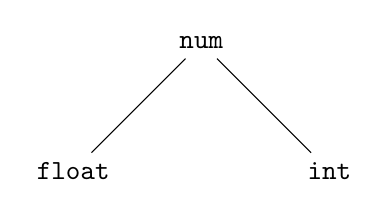
\begin{tikzpicture}[node distance=2.3cm]
    \node(num) 												{\texttt{num}};
    \node(int)		[below right of=num]			{\texttt{int}};
    \node(float)					[below left of=num] 			{\texttt{float}};
    \draw (num)      -- (int);
    \draw (num)      -- (float);
  \end{tikzpicture}
  \caption{Orden parcial entre los tipos}
  \label{subt1}
\end{figure}

Luego, introduce los tipos \texttt{meet} y \texttt{join}, que corresponden a la máxima cota inferior (ínfimo) y a la mínima cota superior (súpremo) entre dos tipos, respectivamente. Pese a que Cardelli no considera una inferencia basada en constraints, se puede aplicar este enfoque para la resolución de constraints de subtyping. En efecto, Pottier~\cite{pottier:inria-00073205} y Sekiguchi~\cite{sekiguchi} presentan sistemas de inferencia basados en constraints, con tipos equivalentes a los \texttt{meet} y \texttt{join} de Cardelli.

Las operaciones \texttt{meet} y \texttt{join} tienen solución si todo par de tipos en el orden parcial tiene un único supremo e ínfimo, lo que se define como lattice. En la figura \ref{subt1}, se debe agregar el tipo \texttt{Bot} para que el orden parcial sea una lattice.

Las reglas para la aplicación de estas operaciones sobre una lattice se muestran en el teorema \ref{teo1}.

\begin{teo} \label{teo1} \normalfont Si \texttt{x}, \texttt{y} y \texttt{z} pertenecen a una lattice de subtyping, se cumple lo siguiente: \\
  \begin{itemize}
    \item \texttt{x <: y}, \texttt{x <: z} $\implies$ \texttt{x <: meet(y, z)}
    \item \texttt{y <: x}, \texttt{z <: x} $\implies$ \texttt{join(y, z) <: x}
  \end{itemize}
\end{teo}

Volviendo al ejemplo \ref{ej2-9}, las constraints generadas se resuelven con la operación \texttt{join} entre \texttt{int} y \texttt{float} debido a la aplicación del teorema \ref{teo1}, lo que da como resultado \texttt{num}.

% Teniendo en cuenta que los distintos sistemas de inferencia propuestos a lo largo del tiempo comparten características, Odersky \textit{et al.}~\cite{odersky} propusieron el framework \texttt{HM(X)}, que entrega un algoritmo de inferencia genérico para un sistema de tipos basado en constraints que cumpla ciertas condiciones.

% Utilizando el framework \texttt{HM(X)}, Pottier y Simonet~\cite{Pottier} presentaron un análisis de control de flujo con inferencia de tipos de seguridad, que hereda todas las buenas propiedades de \texttt{HM(X)}.

\chapter{Especificación del problema}

\input{cap1.tex}
\input{cap2.tex}
\begin{conclusion}

	La desclasificación basada en tipos muestra una conexión entre las relaciones de subtipos de un lenguaje orientado a objetos, y las relaciones de orden que conforman los tipos de seguridad, para proponer un sistema de tipos que cumple una versión relajada de no-interferencia. Con esta propuesta, Cruz \textit{et al.} abordan parcialmente el desafió de integrar los modelos de control de flujo de información con infraestructuras existentes. Este trabajo materializa aquella propuesta, con una implementación para un subconjunto del lenguaje Dart, en conjunto con un sistema de inferencia y una extensión para ambientes de desarrollo.

	A pesar del foco de seguridad que tiene un trabajo de estas características, la formulación del problema de inferencia y el uso de la extensión para integrar los resultados fueron concebidos teniendo al programador en mente, para facilitarle el trabajo y mejorar su experiencia programando, entre otros beneficios. Esta experiencia puede mejorar aún más, agregando nuevas características a la extensión.

	\section*{Trabajo futuro}

	\paragraph{Formalización de inferencia.}En este trabajo se implementó un sistema de inferencia sin demostrar formalmente las propiedades que cumple. Por ejemplo, es deseable demostrar que el sistema propuesto siempre infiere las facetas públicas más ajustadas al uso de las expresiones, o que el sistema de inferencia preserva la propiedad de no-interferencia relajada. En este sentido, es deseable la formalización de la inferencia de tipos de dos facetas, antes de realizar cualquier extensión a este trabajo, cuyo objetivo fue demostrar el uso práctico del enfoque propuesto por Cruz \textit{et al.} Además, es deseable realizar un análisis de la complejidad de los algoritmos propuestos.

	\paragraph{Extensión al subconjunto soportado.}Este trabajo soporta un subconjunto pequeño del lenguaje Dart, lo que no permite probarlo en aplicaciones reales de mayor envergadura. Por ejemplo, la implementación actual no soporta funciones y variables definidas de forma global, excepciones, funciones anónimas, entre otros. Soportar características avanzadas del lenguaje, e implementar la herramienta en otros lenguajes de programación, permitiría posicionar a la herramienta como una alternativa competente de análisis de control de flujo para aplicaciones en producción.

	\paragraph{Características de la extensión para ambientes de desarrollo.}La extensión para ambientes de desarrollo implementada en este trabajo solo muestra los resultados de la inferencia, pero no permite al programador tomar acciones automáticas al respecto. Por ejemplo, sería posible asistir al usuario en la definición de una faceta pública que ha sido declarada, navegar al lugar donde se define una faceta pública al ubicarse en la faceta declarada, definir y declarar una faceta pública basándose en el resultado de la inferencia, entre otros.

	\paragraph{Extensión a polimorfismo.}Una característica interesante a considerar en una posible extensión a este trabajo es el polimorfismo paramétrico. Con esto, es posible la definición de estructuras de datos paramétricas en tipos de dos facetas, lo que implica tener polimorfismo en facetas públicas. Además, se pueden definir facetas públicas polimórficas. Por ejemplo, la faceta pública $\mathtt{Eq[X]}\triangleq [\mathtt{eq} : \mathtt{X} \rightarrow \mathtt{Bool}]$ está parametrizada por un tipo \texttt{X}.


\end{conclusion}


% \input{glosario.tex} % opcional

\bibliographystyle{plain}
\bibliography{bibliografia}

% \input{anexo_apendices.tex} % opcionales

\end{document}
